% Options for packages loaded elsewhere
\PassOptionsToPackage{unicode}{hyperref}
\PassOptionsToPackage{hyphens}{url}
\PassOptionsToPackage{dvipsnames,svgnames,x11names}{xcolor}
%
\documentclass[
  11pt,
]{article}

\usepackage{amsmath,amssymb}
\usepackage{setspace}
\usepackage{iftex}
\ifPDFTeX
  \usepackage[T1]{fontenc}
  \usepackage[utf8]{inputenc}
  \usepackage{textcomp} % provide euro and other symbols
\else % if luatex or xetex
  \usepackage{unicode-math}
  \defaultfontfeatures{Scale=MatchLowercase}
  \defaultfontfeatures[\rmfamily]{Ligatures=TeX,Scale=1}
\fi
\usepackage{lmodern}
\ifPDFTeX\else  
    % xetex/luatex font selection
\fi
% Use upquote if available, for straight quotes in verbatim environments
\IfFileExists{upquote.sty}{\usepackage{upquote}}{}
\IfFileExists{microtype.sty}{% use microtype if available
  \usepackage[]{microtype}
  \UseMicrotypeSet[protrusion]{basicmath} % disable protrusion for tt fonts
}{}
\makeatletter
\@ifundefined{KOMAClassName}{% if non-KOMA class
  \IfFileExists{parskip.sty}{%
    \usepackage{parskip}
  }{% else
    \setlength{\parindent}{0pt}
    \setlength{\parskip}{6pt plus 2pt minus 1pt}}
}{% if KOMA class
  \KOMAoptions{parskip=half}}
\makeatother
\usepackage{xcolor}
\setlength{\emergencystretch}{3em} % prevent overfull lines
\setcounter{secnumdepth}{-\maxdimen} % remove section numbering
% Make \paragraph and \subparagraph free-standing
\ifx\paragraph\undefined\else
  \let\oldparagraph\paragraph
  \renewcommand{\paragraph}[1]{\oldparagraph{#1}\mbox{}}
\fi
\ifx\subparagraph\undefined\else
  \let\oldsubparagraph\subparagraph
  \renewcommand{\subparagraph}[1]{\oldsubparagraph{#1}\mbox{}}
\fi

\usepackage{color}
\usepackage{fancyvrb}
\newcommand{\VerbBar}{|}
\newcommand{\VERB}{\Verb[commandchars=\\\{\}]}
\DefineVerbatimEnvironment{Highlighting}{Verbatim}{commandchars=\\\{\}}
% Add ',fontsize=\small' for more characters per line
\usepackage{framed}
\definecolor{shadecolor}{RGB}{241,243,245}
\newenvironment{Shaded}{\begin{snugshade}}{\end{snugshade}}
\newcommand{\AlertTok}[1]{\textcolor[rgb]{0.68,0.00,0.00}{#1}}
\newcommand{\AnnotationTok}[1]{\textcolor[rgb]{0.37,0.37,0.37}{#1}}
\newcommand{\AttributeTok}[1]{\textcolor[rgb]{0.40,0.45,0.13}{#1}}
\newcommand{\BaseNTok}[1]{\textcolor[rgb]{0.68,0.00,0.00}{#1}}
\newcommand{\BuiltInTok}[1]{\textcolor[rgb]{0.00,0.23,0.31}{#1}}
\newcommand{\CharTok}[1]{\textcolor[rgb]{0.13,0.47,0.30}{#1}}
\newcommand{\CommentTok}[1]{\textcolor[rgb]{0.37,0.37,0.37}{#1}}
\newcommand{\CommentVarTok}[1]{\textcolor[rgb]{0.37,0.37,0.37}{\textit{#1}}}
\newcommand{\ConstantTok}[1]{\textcolor[rgb]{0.56,0.35,0.01}{#1}}
\newcommand{\ControlFlowTok}[1]{\textcolor[rgb]{0.00,0.23,0.31}{#1}}
\newcommand{\DataTypeTok}[1]{\textcolor[rgb]{0.68,0.00,0.00}{#1}}
\newcommand{\DecValTok}[1]{\textcolor[rgb]{0.68,0.00,0.00}{#1}}
\newcommand{\DocumentationTok}[1]{\textcolor[rgb]{0.37,0.37,0.37}{\textit{#1}}}
\newcommand{\ErrorTok}[1]{\textcolor[rgb]{0.68,0.00,0.00}{#1}}
\newcommand{\ExtensionTok}[1]{\textcolor[rgb]{0.00,0.23,0.31}{#1}}
\newcommand{\FloatTok}[1]{\textcolor[rgb]{0.68,0.00,0.00}{#1}}
\newcommand{\FunctionTok}[1]{\textcolor[rgb]{0.28,0.35,0.67}{#1}}
\newcommand{\ImportTok}[1]{\textcolor[rgb]{0.00,0.46,0.62}{#1}}
\newcommand{\InformationTok}[1]{\textcolor[rgb]{0.37,0.37,0.37}{#1}}
\newcommand{\KeywordTok}[1]{\textcolor[rgb]{0.00,0.23,0.31}{#1}}
\newcommand{\NormalTok}[1]{\textcolor[rgb]{0.00,0.23,0.31}{#1}}
\newcommand{\OperatorTok}[1]{\textcolor[rgb]{0.37,0.37,0.37}{#1}}
\newcommand{\OtherTok}[1]{\textcolor[rgb]{0.00,0.23,0.31}{#1}}
\newcommand{\PreprocessorTok}[1]{\textcolor[rgb]{0.68,0.00,0.00}{#1}}
\newcommand{\RegionMarkerTok}[1]{\textcolor[rgb]{0.00,0.23,0.31}{#1}}
\newcommand{\SpecialCharTok}[1]{\textcolor[rgb]{0.37,0.37,0.37}{#1}}
\newcommand{\SpecialStringTok}[1]{\textcolor[rgb]{0.13,0.47,0.30}{#1}}
\newcommand{\StringTok}[1]{\textcolor[rgb]{0.13,0.47,0.30}{#1}}
\newcommand{\VariableTok}[1]{\textcolor[rgb]{0.07,0.07,0.07}{#1}}
\newcommand{\VerbatimStringTok}[1]{\textcolor[rgb]{0.13,0.47,0.30}{#1}}
\newcommand{\WarningTok}[1]{\textcolor[rgb]{0.37,0.37,0.37}{\textit{#1}}}

\providecommand{\tightlist}{%
  \setlength{\itemsep}{0pt}\setlength{\parskip}{0pt}}\usepackage{longtable,booktabs,array}
\usepackage{calc} % for calculating minipage widths
% Correct order of tables after \paragraph or \subparagraph
\usepackage{etoolbox}
\makeatletter
\patchcmd\longtable{\par}{\if@noskipsec\mbox{}\fi\par}{}{}
\makeatother
% Allow footnotes in longtable head/foot
\IfFileExists{footnotehyper.sty}{\usepackage{footnotehyper}}{\usepackage{footnote}}
\makesavenoteenv{longtable}
\usepackage{graphicx}
\makeatletter
\def\maxwidth{\ifdim\Gin@nat@width>\linewidth\linewidth\else\Gin@nat@width\fi}
\def\maxheight{\ifdim\Gin@nat@height>\textheight\textheight\else\Gin@nat@height\fi}
\makeatother
% Scale images if necessary, so that they will not overflow the page
% margins by default, and it is still possible to overwrite the defaults
% using explicit options in \includegraphics[width, height, ...]{}
\setkeys{Gin}{width=\maxwidth,height=\maxheight,keepaspectratio}
% Set default figure placement to htbp
\makeatletter
\def\fps@figure{htbp}
\makeatother

\makeatletter
\makeatother
\makeatletter
\makeatother
\makeatletter
\@ifpackageloaded{caption}{}{\usepackage{caption}}
\AtBeginDocument{%
\ifdefined\contentsname
  \renewcommand*\contentsname{Table of contents}
\else
  \newcommand\contentsname{Table of contents}
\fi
\ifdefined\listfigurename
  \renewcommand*\listfigurename{List of Figures}
\else
  \newcommand\listfigurename{List of Figures}
\fi
\ifdefined\listtablename
  \renewcommand*\listtablename{List of Tables}
\else
  \newcommand\listtablename{List of Tables}
\fi
\ifdefined\figurename
  \renewcommand*\figurename{Figure}
\else
  \newcommand\figurename{Figure}
\fi
\ifdefined\tablename
  \renewcommand*\tablename{Table}
\else
  \newcommand\tablename{Table}
\fi
}
\@ifpackageloaded{float}{}{\usepackage{float}}
\floatstyle{ruled}
\@ifundefined{c@chapter}{\newfloat{codelisting}{h}{lop}}{\newfloat{codelisting}{h}{lop}[chapter]}
\floatname{codelisting}{Listing}
\newcommand*\listoflistings{\listof{codelisting}{List of Listings}}
\makeatother
\makeatletter
\@ifpackageloaded{caption}{}{\usepackage{caption}}
\@ifpackageloaded{subcaption}{}{\usepackage{subcaption}}
\makeatother
\makeatletter
\@ifpackageloaded{tcolorbox}{}{\usepackage[skins,breakable]{tcolorbox}}
\makeatother
\makeatletter
\@ifundefined{shadecolor}{\definecolor{shadecolor}{rgb}{.97, .97, .97}}
\makeatother
\makeatletter
\makeatother
\makeatletter
\makeatother
\ifLuaTeX
  \usepackage{selnolig}  % disable illegal ligatures
\fi
\IfFileExists{bookmark.sty}{\usepackage{bookmark}}{\usepackage{hyperref}}
\IfFileExists{xurl.sty}{\usepackage{xurl}}{} % add URL line breaks if available
\urlstyle{same} % disable monospaced font for URLs
\hypersetup{
  pdftitle={Análisis Descriptivo de la Autopercepción Social y la Satisfacción Democrática en Chile (ELSOC 2016)},
  pdfauthor={Violeta Paz Rivera Sepúlveda y Benjamín Felipe Sepúlveda},
  colorlinks=true,
  linkcolor={blue},
  filecolor={Maroon},
  citecolor={Blue},
  urlcolor={Blue},
  pdfcreator={LaTeX via pandoc}}

\title{Análisis Descriptivo de la Autopercepción Social y la
Satisfacción Democrática en Chile (ELSOC 2016)}
\author{Violeta Paz Rivera Sepúlveda y Benjamín Felipe Sepúlveda}
\date{}

\begin{document}
\maketitle
\ifdefined\Shaded\renewenvironment{Shaded}{\begin{tcolorbox}[frame hidden, breakable, boxrule=0pt, enhanced, interior hidden, sharp corners, borderline west={3pt}{0pt}{shadecolor}]}{\end{tcolorbox}}\fi

\setstretch{1.5}
\hypertarget{introducciuxf3n}{%
\section{Introducción}\label{introducciuxf3n}}

En el contexto chileno actual, marcado por transformaciones políticas,
desigualdades persistentes y un creciente distanciamiento entre
ciudadanía e instituciones, se vuelve relevante comprender cómo las
personas se perciben a sí mismas dentro del entramado social. Esta
percepción subjetiva de la posición social puede incidir en diversas
dimensiones de la vida, incluyendo las actitudes hacia la democracia y
su evaluación.

Desde la sociología, resulta clave estudiar estos fenómenos considerando
no solo las estructuras objetivas (como ingreso o educación), sino
también las representaciones que las personas construyen respecto a su
lugar en la sociedad. El presente estudio busca explorar la relación
entre la \textbf{autoubicación social subjetiva} y la
\textbf{satisfacción con la democracia} en Chile.

Entendemos por autoubicación social la forma en que los/as individuos/as
se posicionan en una escala de estatus social percibido, medida del 1
(posición más baja) al 10 (más alta). Por su parte, la satisfacción con
la democracia remite a la valoración que la ciudadanía hace del
funcionamiento del régimen democrático, considerado un indicador clave
de legitimidad política.

La relevancia sociológica de este estudio radica en que diversas
investigaciones han mostrado que la percepción subjetiva del estatus
social influye en la forma en que las personas se relacionan con
instituciones, política y bienestar general (Manstead, 2018; Kraus et
al., 2012). En contextos de alta desigualdad como el chileno, esta
percepción puede alejarse de indicadores objetivos, pero aún así tener
efectos significativos sobre las actitudes cívicas.

Nuestra hipótesis plantea que: \textbf{a medida que aumenta la
autoubicación social subjetiva (es decir, las personas se sienten en una
mejor posición), tiende a aumentar la satisfacción con la democracia}.
Esta relación puede explicarse por una mayor sensación de integración y
reconocimiento social entre quienes se perciben en una mejor posición.

La fuente de datos utilizada es la Encuesta Longitudinal Social de Chile
(ELSOC), Ola 1 del año 2016. Esta encuesta es representativa a nivel
nacional y permite analizar actitudes y percepciones sociales de la
población adulta en el país.

\begin{Shaded}
\begin{Highlighting}[]
\CommentTok{\# Carga Librerías {-}{-}{-}{-}{-}{-}{-}{-}{-}{-}{-}{-}{-}{-}{-}{-}{-}{-}{-}{-}{-}{-}{-}{-}{-}{-}{-}{-}{-}{-}{-}{-}{-}{-}{-}{-}{-}{-}{-}{-}{-}{-}{-}{-}{-}{-}{-}{-}{-}{-}{-}{-}{-}{-}{-}{-}{-}{-}{-}{-}{-}{-}}

\FunctionTok{library}\NormalTok{(pacman)}
\NormalTok{pacman}\SpecialCharTok{::}\FunctionTok{p\_load}\NormalTok{(tidyverse,  }
\NormalTok{               car,}
\NormalTok{               stargazer,}
\NormalTok{               sjlabelled,}
\NormalTok{               sjPlot,      }
\NormalTok{               confintr,    }
\NormalTok{               gginference,  }
\NormalTok{               rempsyc,     }
\NormalTok{               broom,       }
\NormalTok{               sjmisc,      }
\NormalTok{               dplyr,}
\NormalTok{               knitr,}
\NormalTok{               flextable)           }

\FunctionTok{options}\NormalTok{(}\AttributeTok{scipen =} \DecValTok{999}\NormalTok{) }\CommentTok{\# para desactivar notacion cientifica}
\FunctionTok{rm}\NormalTok{(}\AttributeTok{list =} \FunctionTok{ls}\NormalTok{()) }\CommentTok{\# para limpiar el entorno de trabajo}


\CommentTok{\# Carga datos {-}{-}{-}{-}{-}{-}{-}{-}{-}{-}{-}{-}{-}{-}{-}{-}{-}{-}{-}{-}{-}{-}{-}{-}{-}{-}{-}{-}{-}{-}{-}{-}{-}{-}{-}{-}{-}{-}{-}{-}{-}{-}{-}{-}{-}{-}{-}{-}{-}{-}{-}{-}{-}{-}{-}{-}{-}{-}{-}{-}{-}{-}{-}{-}{-}{-}}

\FunctionTok{load}\NormalTok{(}\StringTok{"input/ELSOC\_Long.RData"}\NormalTok{)}
\end{Highlighting}
\end{Shaded}

\hypertarget{selecciuxf3n-de-variables-y-justificaciuxf3n-socioluxf3gica}{%
\section{Selección de variables y justificación
sociológica}\label{selecciuxf3n-de-variables-y-justificaciuxf3n-socioluxf3gica}}

\textbf{1. Autoubicación en la sociedad chilena
(\texttt{autoubi\_socie})}\\
Esta variable recoge la percepción subjetiva de estatus social en una
escala del 1 al 10. Su inclusión es central, ya que permite captar cómo
las personas evalúan su lugar en la estructura social, considerando
factores no siempre capturados por indicadores objetivos (como el
capital cultural o simbólico). En estudios previos, esta percepción ha
mostrado ser predictiva de bienestar, confianza y actitudes políticas
(Operario et al., 2004; Kraus et al., 2012).

\textbf{2. Satisfacción con el funcionamiento de la democracia
(\texttt{satis\_demo})}\\
Se trata de una variable ordinal que refleja la evaluación de las
personas sobre la democracia chilena. Esta medida es clave para evaluar
el vínculo entre ciudadanía e instituciones, especialmente en un país
donde los niveles de confianza política han sido históricamente bajos.
La sociología política ha demostrado que la percepción de justicia y
representación se relaciona estrechamente con el nivel de satisfacción
democrática (Norris, 2011).

\begin{Shaded}
\begin{Highlighting}[]
\DocumentationTok{\#\# Filtrar y seleccionar {-}{-}{-}{-}{-}{-}{-}{-}{-}{-}{-}{-}{-}{-}{-}{-}{-}{-}{-}{-}{-}{-}{-}{-}{-}{-}{-}{-}{-}{-}{-}{-}{-}{-}{-}{-}{-}{-}{-}{-}{-}{-}{-}{-}{-}{-}{-}{-}{-}{-}{-}{-}{-}{-}{-}}
\NormalTok{data }\OtherTok{\textless{}{-}}\NormalTok{ elsoc\_long\_2016\_2022 }\SpecialCharTok{\%\textgreater{}\%} 
  \FunctionTok{filter}\NormalTok{(ola}\SpecialCharTok{==}\DecValTok{1}\NormalTok{) }\SpecialCharTok{\%\textgreater{}\%}
  \FunctionTok{select}\NormalTok{(d01\_01,c01)}

\DocumentationTok{\#\# Remover NA\textquotesingle{}s {-}{-}{-}{-}{-}{-}{-}{-}{-}{-}{-}{-}{-}{-}{-}{-}{-}{-}{-}{-}{-}{-}{-}{-}{-}{-}{-}{-}{-}{-}{-}{-}{-}{-}{-}{-}{-}{-}{-}{-}{-}{-}{-}{-}{-}{-}{-}{-}{-}{-}{-}{-}{-}{-}{-}{-}{-}{-}{-}{-}{-}{-}{-}{-}}
\NormalTok{data }\OtherTok{\textless{}{-}}\NormalTok{ data }\SpecialCharTok{\%\textgreater{}\%} 
  \FunctionTok{set\_na}\NormalTok{(., }\AttributeTok{na =} \FunctionTok{c}\NormalTok{(}\SpecialCharTok{{-}}\DecValTok{888}\NormalTok{, }\SpecialCharTok{{-}}\DecValTok{999}\NormalTok{)) }\SpecialCharTok{\%\textgreater{}\%} 
  \FunctionTok{na.omit}\NormalTok{()}

\CommentTok{\#Reetiquetado de variables}

\NormalTok{data }\OtherTok{\textless{}{-}}\NormalTok{ data }\SpecialCharTok{\%\textgreater{}\%} \FunctionTok{rename}\NormalTok{(}\StringTok{"satis\_demo"}\OtherTok{=}\NormalTok{c01,          }\CommentTok{\#Satisfacción con el funcionamiento de la democracia.}
                        \StringTok{"autoubi\_socie"}\OtherTok{=}\NormalTok{d01\_01) }

\NormalTok{data}\SpecialCharTok{$}\NormalTok{satis\_demo }\OtherTok{\textless{}{-}} \FunctionTok{set\_label}\NormalTok{(data}\SpecialCharTok{$}\NormalTok{satis\_demo, }\AttributeTok{label =} \StringTok{"Satisfacción con el funcionamiento de la democracia"}\NormalTok{)}
\NormalTok{data}\SpecialCharTok{$}\NormalTok{autoubi\_socie }\OtherTok{\textless{}{-}} \FunctionTok{set\_label}\NormalTok{(data}\SpecialCharTok{$}\NormalTok{autoubi\_socie, }\AttributeTok{label =} \StringTok{"Autoubicación en la sociedad chilena"}\NormalTok{)}
\end{Highlighting}
\end{Shaded}

\hypertarget{visualizaciuxf3n-de-resultados}{%
\section{Visualización de
resultados}\label{visualizaciuxf3n-de-resultados}}

A continuación, se presenta una tabla descriptiva que resume las
principales medidas estadísticas para las variables de interés en este
estudio: autoubicación social subjetiva y satisfacción con la
democracia.

\begin{Shaded}
\begin{Highlighting}[]
\FunctionTok{stargazer}\NormalTok{(data,}\AttributeTok{type=} \StringTok{"text"}\NormalTok{)}
\end{Highlighting}
\end{Shaded}

\begin{verbatim}

==========================================
Statistic       N   Mean  St. Dev. Min Max
------------------------------------------
autoubi_socie 2,790 4.352  1.555    0  10 
satis_demo    2,790 1.995  1.084    1   5 
------------------------------------------
\end{verbatim}

\begin{verbatim}
\end{verbatim}

\begin{verbatim}
\end{verbatim}

\hypertarget{gruxe1ficos}{%
\section{Gráficos}\label{gruxe1ficos}}

Teniendo nuestra tabla descriptiva como punto de partida, realizaremos a
continuación una serie de gráficos que nos permitirán visualizar la
distribución de las variables de interés. Estas representaciones
gráficas facilitarán la comprensión de los patrones presentes en los
datos y apoyarán la interpretación de los resultados obtenidos.

\textbf{Gráfico 1: Distribución de la autoubicación social subjetiva}

A continuación, se muestra un gráfico que representa la distribución de
la variable~\emph{autoubicación social subjetiva}. Este gráfico permite
observar cómo se concentran las respuestas a lo largo de la escala de 0
a 10, identificando posibles asimetrías, acumulaciones o extremos en la
percepción del estatus social.

\begin{Shaded}
\begin{Highlighting}[]
\FunctionTok{ggplot}\NormalTok{(data, }\FunctionTok{aes}\NormalTok{(}\AttributeTok{x =}\NormalTok{ autoubi\_socie)) }\SpecialCharTok{+}
  \FunctionTok{geom\_bar}\NormalTok{(}\AttributeTok{fill =} \StringTok{"\#F4A7B9"}\NormalTok{) }\SpecialCharTok{+}  \CommentTok{\# rosado pastel}
  \FunctionTok{labs}\NormalTok{(}
    \AttributeTok{title =} \StringTok{"Autoubicación en la sociedad chilena"}\NormalTok{,}
    \AttributeTok{x =} \StringTok{"Ubicación social (1 = más bajo, 10 = más alto)"}\NormalTok{,}
    \AttributeTok{y =} \StringTok{"Frecuencia"}
\NormalTok{  ) }\SpecialCharTok{+}
  \FunctionTok{theme\_minimal}\NormalTok{(}\AttributeTok{base\_family =} \StringTok{"sans"}\NormalTok{) }\SpecialCharTok{+}
  \FunctionTok{theme}\NormalTok{(}\AttributeTok{plot.title =} \FunctionTok{element\_text}\NormalTok{(}\AttributeTok{face =} \StringTok{"bold"}\NormalTok{))}
\end{Highlighting}
\end{Shaded}

\begin{figure}[H]

{\centering 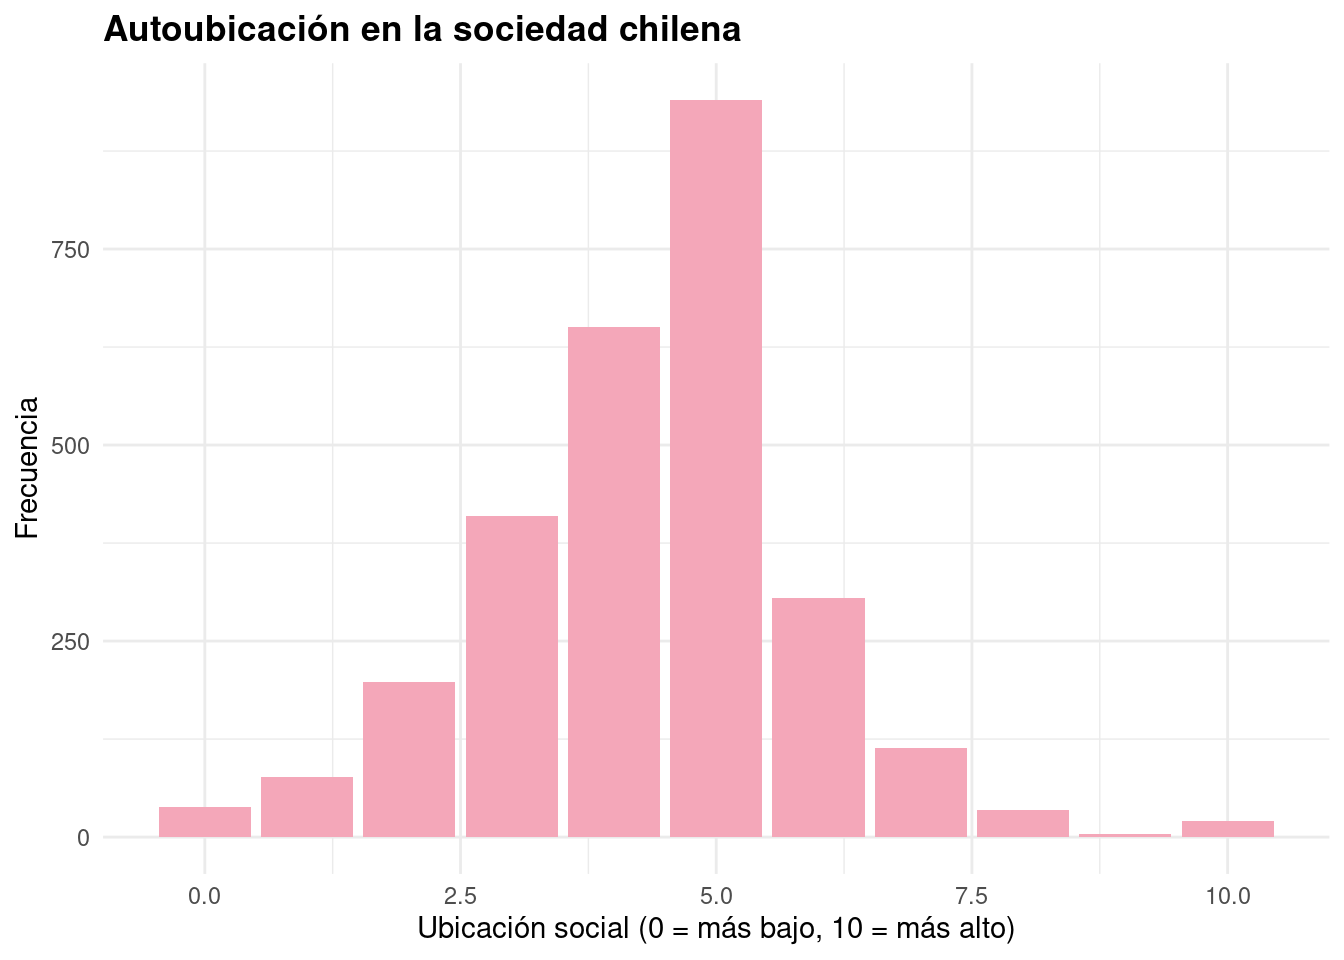
\includegraphics{eLVERDADEROr_files/figure-pdf/unnamed-chunk-4-1.pdf}

}

\end{figure}

Grafico 2

El siguiente gráfico muestra la distribución de la
variable~\emph{satisfacción con la democracia}. Dado que esta se mide en
una escala de 1 a 5, el gráfico facilita identificar tendencias
generales en la valoración que hace la ciudadanía del funcionamiento
democrático en Chile.

\begin{Shaded}
\begin{Highlighting}[]
\FunctionTok{ggplot}\NormalTok{(data, }\FunctionTok{aes}\NormalTok{(}\AttributeTok{x =}\NormalTok{ satis\_demo)) }\SpecialCharTok{+}
  \FunctionTok{geom\_bar}\NormalTok{(}\AttributeTok{fill =} \StringTok{"\#CBAACB"}\NormalTok{) }\SpecialCharTok{+}  \CommentTok{\# lila pastel}
  \FunctionTok{labs}\NormalTok{(}
    \AttributeTok{title =} \StringTok{"Satisfacción con la democracia"}\NormalTok{,}
    \AttributeTok{x =} \StringTok{"Nivel de satisfacción"}\NormalTok{,}
    \AttributeTok{y =} \StringTok{"Frecuencia"}
\NormalTok{  ) }\SpecialCharTok{+}
  \FunctionTok{theme\_minimal}\NormalTok{(}\AttributeTok{base\_family =} \StringTok{"sans"}\NormalTok{) }\SpecialCharTok{+}
  \FunctionTok{theme}\NormalTok{(}\AttributeTok{axis.text.x =} \FunctionTok{element\_text}\NormalTok{(}\AttributeTok{angle =} \DecValTok{25}\NormalTok{, }\AttributeTok{hjust =} \DecValTok{1}\NormalTok{),}
        \AttributeTok{plot.title =} \FunctionTok{element\_text}\NormalTok{(}\AttributeTok{face =} \StringTok{"bold"}\NormalTok{))}
\end{Highlighting}
\end{Shaded}

\begin{figure}[H]

{\centering 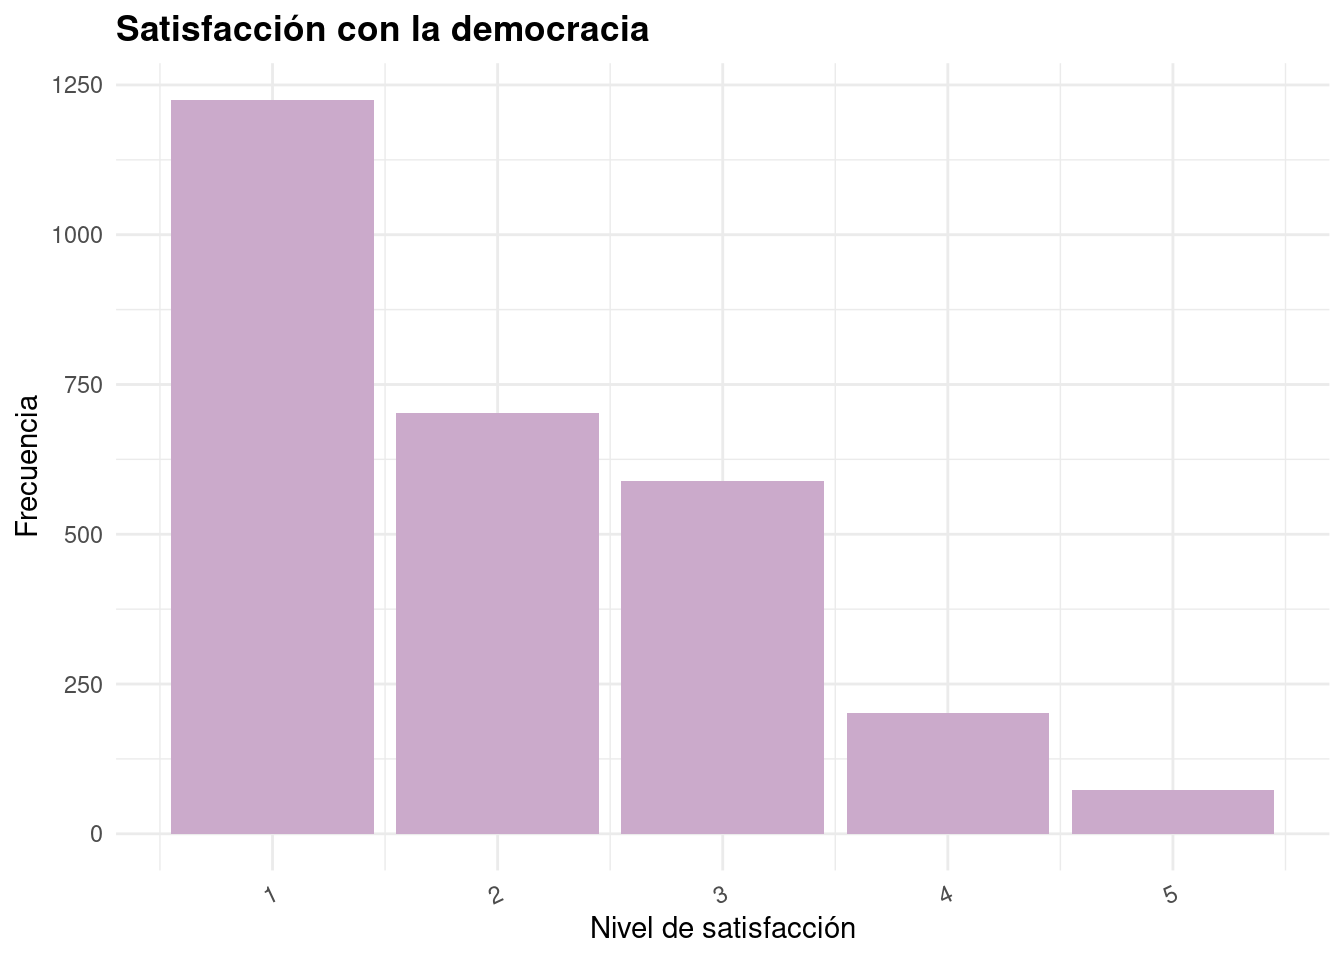
\includegraphics{eLVERDADEROr_files/figure-pdf/unnamed-chunk-5-1.pdf}

}

\end{figure}

\hypertarget{interpretaciuxf3n-de-resultados}{%
\section{Interpretación de
resultados}\label{interpretaciuxf3n-de-resultados}}

Los resultados descriptivos muestran que la autoubicación social
subjetiva presenta un promedio de~\textbf{4.35}~en una escala de 0 a 10,
con una desviación estándar de~\textbf{1.56}. Esto sugiere que, en
promedio, las personas se perciben en una posición intermedia-baja
dentro de la escala social, con cierta dispersión en las respuestas. El
mínimo reportado fue~\textbf{0}~y el máximo~\textbf{10}, lo que indica
que se utilizaron todos los niveles posibles de la escala.

Por otro lado, la satisfacción con la democracia tiene un promedio
de~\textbf{1.99}~en una escala de 1 a 5, con una desviación estándar
de~\textbf{1.08}. Este resultado indica un nivel de satisfacción
relativamente bajo entre las personas encuestadas, con una dispersión
moderada. Aunque el valor máximo observado fue~\textbf{5}, el promedio
cercano a~\textbf{2}~sugiere una tendencia general hacia la
insatisfacción con el funcionamiento de la democracia en Chile al
momento de la medición.

En conjunto, los datos muestran que tanto la percepción del estatus
social como la satisfacción con la democracia tienden a ubicarse en
niveles bajos, lo que podría estar reflejando tensiones sociales
importantes y una desconexión entre ciudadanía e instituciones. Estos
resultados dan pie a profundizar en el análisis de la relación entre
ambas variables.



\end{document}
